% !TEX TS-program = pdflatex
% !TEX encoding = UTF-8 Unicode

%tells you if you use obsolete packages
%\RequirePackage[l2tabu,orthodox]{nag}

\documentclass[]{article}

\usepackage[utf8]{inputenc} % set input encoding (not needed with XeLaTeX)

%%% PAGE DIMENSIONS
\usepackage{geometry} % to change the page dimensions
\geometry{a4paper} % or letterpaper (US) or a5paper or....
% \geometry{margin=2in} % for example, change the margins to 2 inches all round
% \geometry{landscape} % set up the page for landscape
%   read geometry.pdf for detailed page layout information

\usepackage{graphicx} % support the \includegraphics command and options

% \usepackage[parfill]{parskip} % Activate to begin paragraphs with an empty line rather than an indent

%%% PACKAGES
\usepackage{booktabs} % for much better looking tables
\usepackage{array} % for better arrays (eg matrices) in maths
\usepackage{paralist} % very flexible & customisable lists (eg. enumerate/itemize, etc.)
\usepackage{verbatim} % adds environment for commenting out blocks of text & for better verbatim
\usepackage{subfig} % make it possible to include more than one captioned figure/table in a single float
\usepackage{microtype} %makes awesome kerning and punctuation come half way out the edge of the text
\usepackage{listings} %for code listings
\usepackage{color} %for colored syntax highligting
\usepackage{rotating}
\usepackage{pdflscape}
\usepackage[]{algorithm2e}
\usepackage{multirow}
\usepackage{float}
\usepackage{mathtools}
\usepackage{amssymb}

\usepackage{caption}
% \captionsetup[subfigure]{format=subfig,labelsep=colon,labelformat=simple}
% \usepackage{subcaption}


%%% Code listing
\definecolor{mygreen}{rgb}{0,0.6,0}
\definecolor{mygray}{rgb}{0.5,0.5,0.5}
\definecolor{mymauve}{rgb}{0.58,0,0.82}
\lstset{
basicstyle=\footnotesize\ttfamily,
commentstyle=\color{mygreen},
keywordstyle=\color{blue},
numberstyle=\tiny\color{mygray},
numbers=left,
tabsize=2,
frame=tb,
aboveskip=3mm,
belowskip=3mm,
breaklines=true,
breakatwhitespace=true,
showstringspaces=false,
columns=flexible
}

% to include a file as a listing: \lstinputlisting{intio.c}
% inline listing: \begin{lstlisting}[frame=single]

%%% HEADERS & FOOTERS
\usepackage{fancyhdr} % This should be set AFTER setting up the page geometry
\pagestyle{fancy} % options: empty , plain , fancy
\renewcommand{\headrulewidth}{0pt} % customise the layout...
\lhead{}\chead{}\rhead{}
\lfoot{}\cfoot{\thepage}\rfoot{}

%%% ToC (table of contents) APPEARANCE
\usepackage[nottoc,notlof,notlot]{tocbibind} % Put the bibliography in the ToC
% \usepackage[titles,subfigure]{tocloft} % Alter the style of the Table of Contents
%\renewcommand{\cftsecfont}{\rmfamily\mdseries\upshape}
%\renewcommand{\cftsecpagefont}{\rmfamily\mdseries\upshape} % No bold!
\usepackage{hyperref} % use hyperlinked ToC
\hypersetup{colorlinks=true, linkcolor=black, citecolor=black, filecolor=black, urlcolor=black}
\graphicspath{ {ImageLib/}{other_folder/}{third_folder/} }

\usepackage[printonlyused]{acronym}

%%%-------------------------------------------------------------------


\title{Third Year Group Project \\ State Estimation for Indoor Environments}
\author{Oskar Weigl, Ryan Savatski, Thomas Morrison, Chinemelu Ezeh, Joshua Elsdon}
\begin{document}
\maketitle
\center{\textbf{\large{\emph{"...a profound trust in the advances of science."}	}}}

\abstract{
A Lovely Abstract full of insight and long words that makes it apparent we did lots of stuff 
\tableofcontents
\clearpage

\section{Executive Summary} % (fold)
\label{sec:executive_summary}

Summarise things in a summarative way, as if one were producing a summary for an executive. 

% section executive_summary (end)

\section{Introduction}  % (fold)
\label{sec:introduction}
Introduction introducing things in an introductory manner. 
% section introduction (end)

\section{Acronyms} % (fold)
\label{sec:acronyms}
\begin{acronym}
	\acro{EKF}{Extended Kalman Filter}
	\acro{DoF}{Degrees of Freedom}
	\acro{MMSE}{minimum mean square error}
\end{acronym}
% section acronyms (end)

\clearpage

\section{Problem Specification} % (fold)
\label{sec:problem_specification}

\begin{itemize}
	\item What are we trying to achieve
	\item Why is this a good idea to achieve
	\begin{itemize}
		\item why indoor navigation
		\item why are mavrx interested in this
		\item financial rundown (note that mavrx are intersted in a prototype consulting job, not a financial feasability report)
		\item discuss some of mavrx's buisiness model (if we are allowed)
	\end{itemize}
	\item What have other people done in this field
	\begin{itemize}
		\item insert papers here
	\end{itemize}
	\item how are we going to achieve it
	\item Why did we chose to do it that way
	\begin{itemize}
		\item why planes
		\item why xtion
		\item why arndale
		\item why quadcopter
	\end{itemize}
\end{itemize}

% section problem_specification (end)

\section{Sensor Calibration} % (fold)

\begin{figure}
\centering     %%% not \center
\subfloat[MATLAB]{\label{fig:matlabuncal5m}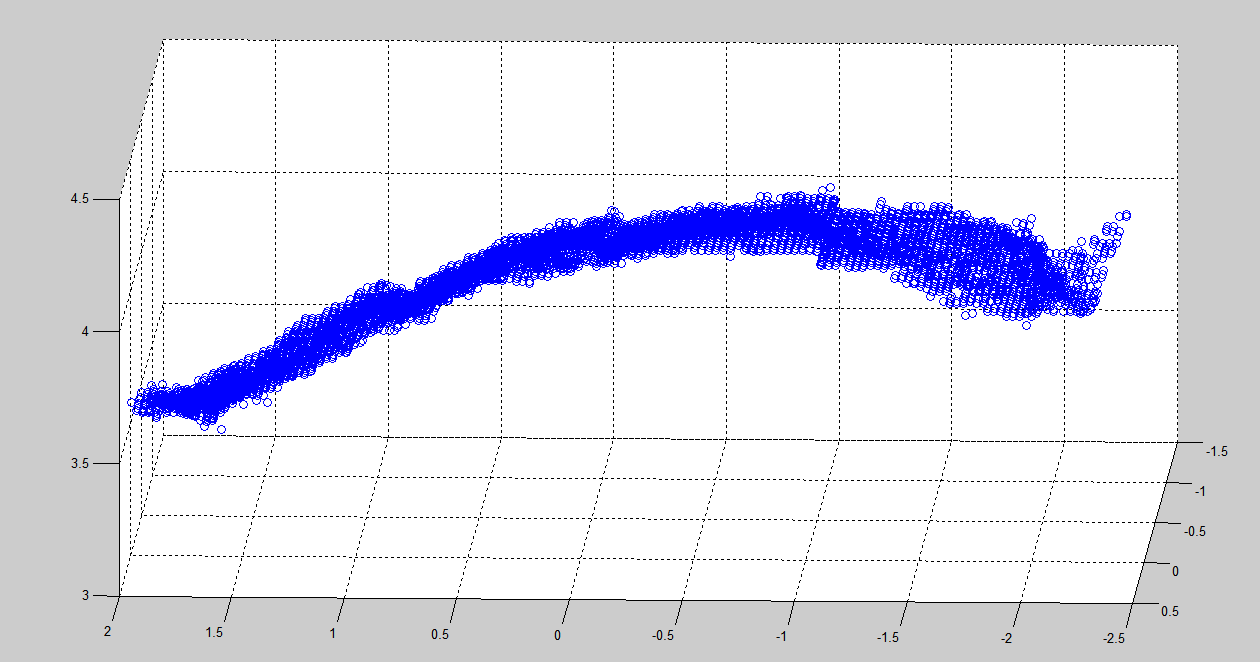
\includegraphics[width=60mm]{uncal5m.PNG}} \,\,\,\,
\subfloat[Colour Point Cloud]{\label{fig:clouduncal5m}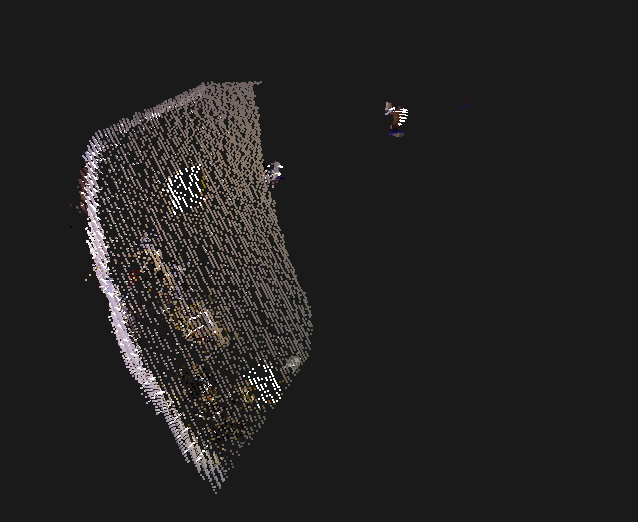
\includegraphics[width=60mm]{wallat6m}}
\caption{Example of the poor calibration of the Xtion sensor}
\label{fig:uncal5m}
\end{figure}


Apon inspecting the output of the Xtion Pro from Asus it became apparent that the accuracy of the data was poor. At short ranges things appeared normal, and planes were indeed flat. At distance more than 2m planes quickly became warped (see Figure~\ref{fig:uncal5m}). This issue will corrupt the accuracy of planes that we extract from the cloud data, rendering the extra sensor of little use. 

To attempt to counteract this issue we collected cloud data from when the sensor is facing a large plane, in this case a wall, at a number of distances (from 0.8m to 4m). This cloud data included lots of objects that are of no use to the calibration, so these data points were written to \verb"NaN" in the analysis to avoid corruption of our results. This was achieved by using the data written to an image file, with the z distance (down range from the camera) encoding the grey-scale. Then, by hand, we masked with black all the unwanted areas. This is then easy to correlate against the original data in MATLAB. 

Figure~\ref{fig:avDist} shows the average measurement across all of the frame for a range of distances. This represents another mode of inaccuracy not only is the image distorted, the distance measurement is very poor. At 4m the average distance measured was 3.32m, which represents a 17\% error. Though the maximum error is 0.941m at 4m, which represents a huge 23.5\% error. 

\begin{figure}[htb]
	\begin{center}
		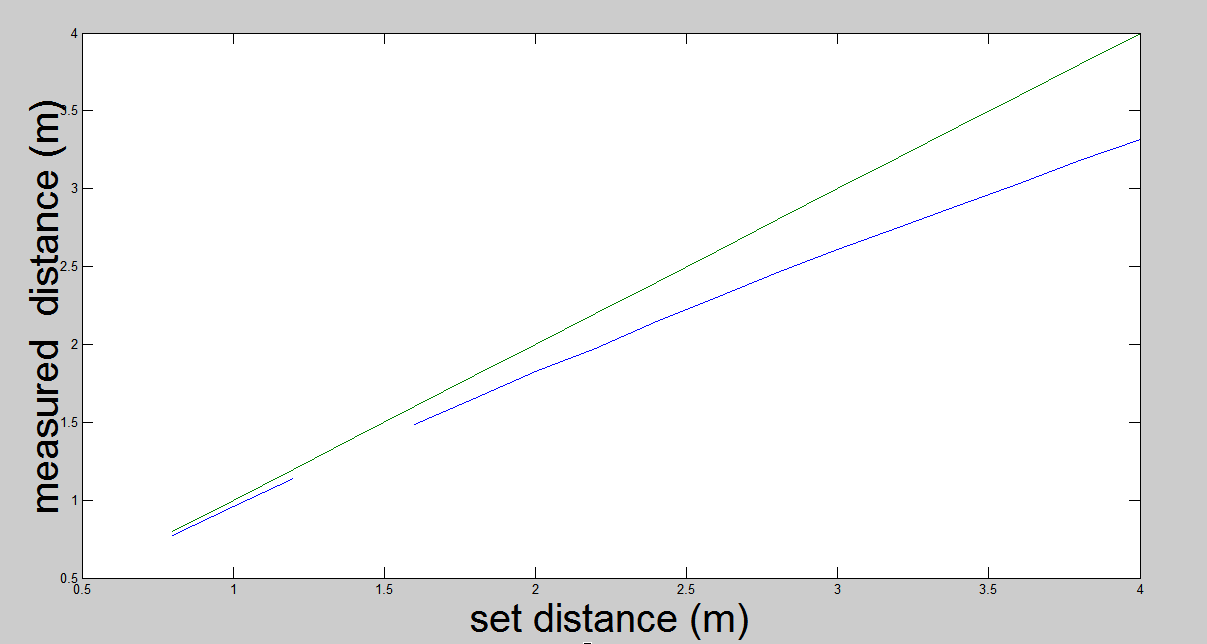
\includegraphics[width = 0.8\textwidth]{avDist}
	\end{center}
	\caption{Measured distance vs set distance. This is the average of all the pixels in the frames at a range of distances, the blue line shows the data. Green shows the target line.}
	\label{fig:avDist}
\end{figure}

Now with the clean data we know that all the data points must belong to a plane with distance to the plane being the calibration distance. For now we assume that the x and y directions are not in need of calibration, as objects in the visualisations do not too distorted in these directions. Therefore we only need to find the difference between measured data and the calibration distance. Mapping these correction vectors into a 3D space that later we can look up in to correct new data. 

In order to have the 3D correction field be continuous we must smooth and interpolate the data in all 3 dimensions. One significant issue is that all of our correction vectors fall into quite thin regions in the 3D space along the z axis, and within those areas the data is very dense in the x and y dimensions. Therefore our task is to preform smoothing in the x and y directions to remove the signal noise and to find a good interpolation scheme looking in the z direction. The interpolation should be smooth to avoid damaging the flatness of planes. 
\clearpage

\section{Feature Extraction} % (fold)
\label{sec:feature_extraction}

% \subsection{Sensor Calibration} % (fold)
% \label{sub:sensor_calibration}

% Multidimensional least squares correction
% measure a plane at a known distance (d)
% least squares establish the observed plane that matches this distance d
% 	(or just least squares the plane first??)
% the distance of each point from the plane is the true calibration vector field projected onto the normal of the observed plane (in the camera's coordinate system)

% subsection sensor_calibration (end)

% section feature_extraction (end)

\clearpage %temp!
\section{EKF} % (fold)
\label{sec:ekf}

To estimate the state of the system we employ an \ac{EKF}. This filter is the nonlinear version of the regular Kalman Filter: the optimal state estimation filter \cite{todo}. This filter will, when supplied with an accurate sytem model, and its statistical properties, provide the state estimate with the minimum mean-squared error.
The \ac{EKF} provides a near-optimal estimate of the system's state by linearising it around the current state estimate. The reason why we need the nonlinear version of the filter is due to the fact that the model includes rotations, which are nonlinear in nature.

% We use a kalman filter... the optimal state estimator
% non linear due to rotations -- ekf
% 	euler vs runge kutta integrator
% 		very complicated linearization equations
% 			can be overcome with unscented kalman
% 		euler is fine if sampling fast enough
% 			if deltaT is small

When deriving the system model, we chose to use an approach that does not rely on an aerodynamic model of the craft, similar to the approach in \cite{OpenPilotPaper}.
This has the advantage that modelling errors are minimised, and the time required for system identification is reduced.
Complex phenomena such as the turbulence caused by the thrust channelled around in the confined space would be close to impossible to model.
As we elect to use a model-less approach
	any system/craft
	decoupled control inputs
	good for our case

As such, while the system is modelled as a six \ac{DoF} rigid body system with Newtonian mechanics, this is not how it is tracked.
As we assume no model of how the control inputs are translated to actuation, we cannot integrate the forces of the system. Instead, we rely on the inertial sensors to inform us of the evolution of the system.

\subsection{Filter Equations} % (fold)
\label{sub:filter_equations}

The filter is based on the following discrete time update model
\begin{align}
	x_k &= f(x_{k-1}, u_{k-1}, w_{k-1}) \notag \\
	y_k &= h(x_k, v_k)
	\label{eqn:system}
\end{align}
where $x_k$ is the state vector at time $k$, $f$ is the state transition function, $u$ is the control input vector at time $k$, $w_k$ is the process noise vector at time $k$, $y_k$ is the measurment vector at time $k$, $h$ is the function that maps the state space to the observed space, and $v_k$ is the measurment noise vector.

The noise in the system is assumed to be gaussian white noise as follows
\begin{align}
	w_k &\sim N(0,Q_k) \notag \\
	v_k &\sim N(0,R_k) \notag \\
	x_0 &\sim N(\hat{x}_0,P_0)
	\label{eqn:noisedef}
\end{align}
where $Q_k$ and $R_k$ are the process noise and measurment noise covariance matricies, at time $k$, respectivly. The initial state estimate error is assumed to be drawn from a normal distrubution with covariance $P_0$.

We define
\begin{align}
	\hat{x}_{k|i} 	&= \mathbb{E}[x_k|y_0 \hdots y_i] \\
	P_{k|i} 		&= \operatorname{cov}(x_k - \hat{x}_{k|i}) \notag \\
					&= \mathbb{E}[ (x_k-\hat{x}_{k|i}) (x_k-\hat{x}_{k|i})^\top | y_0 \hdots y_i]
\end{align}
where $\hat{x}_{k|i}$ is the state estimate at time $k$ given observations of the system output up to and including time $i$, and $P_{k|i}$ is the covariance matrix associated with the error of the state estimate at time $k$ given given observations of the system output up to and including time $i$.

Given the above defenitions and assumptions, we can predict the evolution of the system as follows
\begin{align}
	\hat{x}_{k|k-1} &= f(\hat{x}_{k-1|k-1}, u_{k-1}, \mathbb{E}[w_{k-1}])
	\label{eqn:predictx}
\end{align}
where whe assume that the noise has zero mean:
\begin{align}
	\mathbb{E}[w_{k-1}] &= 0
\end{align}

We transform the state error covariance matrix using a linear approximation to the transformation imposed by the state transition function $f$ as follows:
\begin{align}
	P_{k|k-1} &\approx F_{k-1} P_{k|k} F_{k-1}^\top + G_{k-1} Q_{k-1} G_{k-1}^\top
	\label{eqn:predictP}
\end{align}
where
\begin{align}
	F_{k-1} &= \left . \frac{\partial f}{\partial x} \right \vert _{\hat{x}_{k-1|k-1},u_{k-1}} \\
	G_{k-1} &= \left . \frac{\partial f}{\partial w} \right \vert _{\hat{x}_{k-1|k-1},u_{k-1}}
\end{align}

--------------------------------------------------------------------------------

In order to correct for errors accumulated by the state transition function we incorporate corrections based on measurments made from the output of the system. To do this, we use the \ac{EKF} update equations.
%todo: more flesh here

For each measurement, we compute the expected measurment given our current state estimate using $h$, and compute the difference $z_k$, and estimate the associated covariance matrix using a linear approximation:
\begin{align}
	z_k &= y_k - h(\hat{x}_{k|k-1}, \mathbb{E}[v_k]) \\
	S_k &= \operatorname{cov}(z_k) \notag \\
		&\approx H_k P_{k|k-1} H_k^\top + V_k R_k V_k^\top
\end{align}
where $P$ and $R$ are defined in equation (\ref{eqn:noisedef}), and where whe assume that the noise has zero mean:
\begin{align}
	\mathbb{E}[v_k] &= 0
\end{align}
and where
\begin{align}
	H_{k} &= \left . \frac{\partial h}{\partial x} \right \vert _{\hat{x}_{k|k-1}} \\
	V_{k} &= \left . \frac{\partial h}{\partial v} \right \vert _{\hat{x}_{k|k-1}}
\end{align}

We define the Kalman gain as follows:
\begin{align}
	K_k &= P_{k|k-1} H_k^\top S_k^{-1}
\end{align}
which is the gain that yields the \ac{MMSE} estimates when used \cite{BerkelyCourse}. Using this gain, we compute the updated state estimate as follows:
\begin{align}
	\hat{x}_{k|k} 	&= \hat{x}_{k|k-1} + K_k z_k \\
	P_{k|k} 		&\approx (I - K_k H_k) P_{k|k-1}
\end{align}

% subsubsection filter_equations (end)
\clearpage

\subsection{System Model} % (fold)
\label{sub:system_model}

In order to evaluate the equations from the previous section, we need to establish a model of the system. This involves establishing what 
\begin{align}
	x &= 
	\left[
	\begin{matrix}
		r \\
		v \\
		q \\
		b_\omega \\
		b_a \\
		\pi_0 \\
		\vdots \\
		\pi_{n-1}
	\end{matrix}
	\right]
	&
	\dot{x} &= 
	\left[
	\begin{matrix}
		\dot{r} \\
		\dot{v} \\
		\dot{q} \\
		\dot{b}_\omega \\
		\dot{b}_a \\
		\dot{\pi}_0 \\
		\vdots \\
		\dot{\pi}_{n-1}
	\end{matrix}
	\right]
\end{align}

where $r$ is the position of the craft in the inertial frame, $v$ is the velocity in the inertial frame, $q$ is the quaternion that represents the attitude of the craft: a rotation from the inertial frame to the body frame, $b_\omega$ and $b_a$ represent the gyro and accelerometer bias, respectively. $\pi_0 \hdots \pi_{n-1}$ are the equations of the planes currently stored in the map.
The state vector components are each composed as follows
\begin{align}
	r &= 
	\left[
	\begin{matrix}
		x \\
		y \\
		z
	\end{matrix}
	\right]
	&
	v &=
	\left[
	\begin{matrix}
		\dot{x} \\
		\dot{y} \\
		\dot{z}
	\end{matrix}
	\right]
	&
	q &=
	\left[
	\begin{matrix}
		q_0 \\
		q_1 \\
		q_2 \\
		q_3
	\end{matrix}
	\right]
	&
	b_\omega &=
	\left[
	\begin{matrix}
		b_{\omega_x} \\
		b_{\omega_y} \\
		b_{\omega_z} 
	\end{matrix}
	\right]
	&
	b_a &=
	\left[
	\begin{matrix}
		b_{a_x} \\
		b_{a_y} \\
		b_{a_z} 
	\end{matrix}
	\right]
	&
	\pi &=
	\left[
	\begin{matrix}
		N_x \\
		N_y \\
		N_z \\
		d
	\end{matrix}
	\right]
\end{align}

The derivative of the state vector is computed in order to propagate the state over time.
\begin{align}
	\dot{r} &= v
	&
	\dot{v} &= R_{eb}(q) a
	&
	\dot{q} &= \frac{1}{2}\Xi(q) \omega
	&
	\dot{b}_\omega &= w_{b\omega}
	&
	\dot{b}_a &= w_{ba}
	&
	\dot{\pi} &= 0
\end{align}

where $a$ and $\omega$ are the true body frame accelerations and angular rates, respectively.
$R_{eb}$, the body to earth rotation matrix and $\Xi$ is the matrix that maps the body frame angular rates to the rate of change of quaternion. Both matricies are a function of the current quarternion and are defined below.

\begin{align}
	\omega &= \omega_m + w_\omega - b_\omega &
	a &= a_m + w_a - b_a + g_b
\end{align}
where $a_m$ and $\omega_m$ are the measured accelerations and angular velocities in the body frame, respectively, and $g_b$ is the acceleration due to gravity in the body frame.

The process nosie is defined as follows
\begin{align}
	x &= 
	\left[
	\begin{matrix}
		w_\omega \\
		w_a \\
		w_{ba} \\
		w_{b\omega}
	\end{matrix}
	\right]
\end{align}

$f$ in equation (\ref{eqn:system}) and (\ref{eqn:predictx}) operates in discrete time, but we have established our model in continous time. As such, we perform a first order approximation to the continous time system:
\begin{align}
	f &= I + \Delta T \dot{x}
\end{align}

\begin{align}
	\Xi(q) &=
	\left[
	\begin{matrix}
		-q_1 	& -q_2	& -q_3 	\\
		q_0		& -q_3 	& q_2 	\\
		q_3 	& q_0 	& -q_1 	\\
		-q_2 	& q_1 	& q_0
	\end{matrix}
	\right]
\end{align}

\begin{align}
	\Omega(\omega) &=
	\left[
	\begin{matrix}
		0 			& -\omega_x 	& -\omega_y	& -\omega_z	\\
		\omega_x 	& 0 			& \omega_z 	& -\omega_y \\
		\omega_y 	& -\omega_z 	& 0 		& \omega_x 	\\
		\omega_z 	& \omega_y		& -\omega_x & 0
	\end{matrix}
	\right]
\end{align}

\begin{align}
	\dot{q} 	&= \frac{1}{2} \Omega(\omega) q \\
				&= \frac{1}{2} \Xi(q) \omega
\end{align}

The derivation of the rate of change of the quaternion with respect to angular velocity in the body frame can be found in \cite{MARSlab} (see equation 108). Note that they use the convetion q = q4 + q1i + q2j + q3k, while we use the convention q0 + q1i + q2j + q3k, which is the same convetion used by MATLAB's Aerospace Blockset \cite{MATLABAerospace}, and the OpenPilot implementation \cite{OpenPilotPaper}.
\begin{align}
	q &= q_0 + q_1i + q_2j + q_3k
\end{align}

Rbe (rotation of body with respect to earth)
rotmatrix here.
\begin{align}
	R_{be}(q) &=
	\left[
	\begin{matrix}
		2(q_0^2 + q_1^2) - 1 	& 2(q_1 q_2 + q_0 q_3) 	& 2(q_1 q_3 - q_0 q_2) \\
		2(q_1 q_2 - q_0 q_3) 	& 2(q_0^2 + q_2^2) - 1 	& 2(q_2 q_3 + q_0 q_1) \\
		2(q_1 q_3 + q_0 q_2)	& 2(q_2 q_3 - q_0 q_1)	& 2(q_0^2 + q_3^2) - 1
	\end{matrix}
	\right]
\end{align}

The derivation of the quaternion derived rotation matrix is also shown in \cite{MARSlab} (see equation 91)

as a rotation matrix is orthogonal, we have that
\begin{align}
	R_{eb} &= R_{be}^\top
\end{align}

Linearisation: Jacobians
\begin{align}
	F &= \frac{\partial f}{\partial x} \notag \\
	&=
	I + \frac{\partial \dot{x}}{\partial x} \Delta T \notag \\
	% &= 
	% I_{16+4n \times 16+4n} +
	% \left[
	% \begin{matrix}
	% 	0_{3\times3} 	& I_{3\times3} 	& 0_{3\times4} 	& 0_{3\times3} 		& 0_{3\times3} 	& 0_{3\times4n} \\
	% 	0_{3\times3}		& 0_{3\times3} 	& F_{vq}	& 0_{3\times3} 		& F_{vb_a} 	& 0_{3\times4n} \\
	% 	0_{4\times3}		& 0_{4\times3} 	& F_{qq}	& F_{qb_\omega}	& 0_{4\times3}	& 0_{4\times4n} \\
	% 	0_{3\times3}		& 0_{3\times3}	& 0_{3\times4} 	& 0_{3\times3} 		& 0_{3\times3} 	& 0_{3\times4n} \\
	% 	0_{3\times3}		& 0_{3\times3}	& 0_{3\times4} 	& 0_{3\times3}		& 0_{3\times3}	& 0_{3\times4n} \\
	% 	0_{4n\times3} 		& 0_{4n\times3} 	& 0_{4n\times4} 	& 0_{4n\times3}		& 0_{4n3\times3} 	& 0_{4n\times4n}
	% \end{matrix}
	% \right] 
	% \Delta T
	% \\
	&=
	I_{16+4n \times 16+4n} +
	%\left[
	%\begin{matrix}
	%	I_{16 \times 16} 	& 0_{16 \times 4n} \\
	%	0_{4n \times 16}	& I_{4n \times 4n}
	%\end{matrix}
	%\right]
	%+
	\left[
	\begin{matrix}
		\cdot 		& I_{3x3} 	& \cdot	 	& \cdot		 	& \cdot		& \cdot \\
		\cdot		& \cdot	 	& F_{vq}	& \cdot		 	& F_{vb_a} 	& \cdot \\
		\cdot		& \cdot	 	& F_{qq}	& F_{qb_\omega}	& \cdot		& \cdot \\
		\cdot		& \cdot		& \cdot	 	& \cdot		 	& \cdot		& \cdot \\
		\cdot		& \cdot		& \cdot	 	& \cdot			& \cdot		& \cdot \\
		\cdot		& \cdot		& \cdot	 	& \cdot			& \cdot		& \cdot
		%\dots 		& \vdots	& \vdots 	& \vdots		& \vdots	& \ddots
	\end{matrix}
	\right]
	\Delta T
	\label{eqn:F}
\end{align}
where
\begin{align}
	F_{vq} 	&= 2
	\left[
	\begin{matrix}
		F_{vq1} 	& -F_{vq0} 	& F_{vq3} 	& -F_{vq2} \\
		F_{vq2} 	& -F_{vq3} 	& -F_{vq0} 	& F_{vq1} \\
		F_{vq3} 	& F_{vq2} 	& -F_{vq1} 	& -F_{vq0}
	\end{matrix}
	\right]
\end{align}
where
\begin{align}
	F_{vq(0\cdots3)} &= \Xi(q) a
\end{align}
% that is
% \begin{align}
% 	%a &= a_m - b_a 							\notag 	\\
% 	F_{vq0} &= -q_1 a_x - q_2 a_y - q_3 a_z	\notag 	\\
% 	F_{vq1} &= q_0 a_x - q_3 a_y + q_2 a_z 	\notag	\\
% 	F_{vq2} &= q_3 a_x + q_0 a_y - q_1 a_z \notag	\\
% 	F_{vq3} &= -q_2 a_x + q_1 a_y + q_0 a_z
% \end{align}


%\begin{align}
%	&= 2
%	\left[
%	\begin{matrix}
%		q_0 a_x - q_3 a_y + q_2 a_z 	& q_1 a_x + q_2 a_y + q_3 a_z 	& -q_2 a_x + q_1 a_y + q_0 a_z 	& -q_3 a_x - q_0 a_y + q_1 a_z 	\\
%		q_3 a_x + q_0 a_y - q_1 a_z 	& q_2 a_x - q_1 a_y - q_0 a_z 	& q_1 a_x + q_2 a_y + q_3 a_z 	& q_0 a_x - q_3 a_y + q_2 a_z 	\\
%		-q_2 a_x + q_1 a_y + q_0 a_z 	& q_3 a_x + q_0 a_y - q_1 a_z 	& -q_0 a_x + q_3 a_y - q_2 a_z 	& q_1 a_x + q_2 a_y + q_3 a_z 	\\
%	\end{matrix}
%	\right]
%\end{align}

and further
\begin{align}
	F_{vb_a} &= -R_{eb}(q)
%\end{align}
&
%\begin{align}
	F_{qq}	&= \frac{1}{2} \Omega(\omega)
			 %= \frac{1}{2} \Omega(\omega_m - b_\omega)
%\end{align}
&
%\begin{align}
	F_{qb_\omega} &= -\frac{1}{2} \Xi(q)
\end{align}

We also have that
\begin{align}
	G &= \frac{\partial f}{\partial w} \notag \\
	&=
	\frac{\partial f}{\partial w_k} \Delta T \notag \\
	&=
	\left[
	\begin{matrix}
		\cdot 			& \cdot 	& \cdot 		& \cdot \\
		\cdot 			& G_{vw_a} 	& \cdot 		& \cdot \\
		G_{qw_\omega}	& \cdot 	& \cdot 		& \cdot \\
		\cdot 			& \cdot 	& I_{3\times3}	& \cdot \\
		\cdot 			& \cdot 	& \cdot 		& I_{3\times3}
	\end{matrix}
	\right]
	\Delta T
\end{align}
where $w_k$ is the discrete time noise, and where
\begin{align}
	G_{vw_a} &= R_{eb}(q)
%\end{align}
&
%\begin{align}
	G_{qw_\omega} &= \frac{1}{2} \Xi(q)
%\end{align}
%&
%\begin{align}
%	G_{b_\omega w_{b\omega}} &= I_{3x3}
%&
%	G_{b_a w_{ba}} &= I_{3x3}
\end{align}

% subsection system_model (end)

\subsection{Impementation} % (fold)
\label{sub:impementation}

SerialUpdate: \cite{OpenPilotPaper} and chapter 4.2.2 of \cite{KFBookSerialupdate}
The referenced papers perform an optimization which assumes an entirerly uncorrelated measurment noise covariance matrix. That is the $R$ matrix is purely diagonal.
We, on the other hand, use a measurment model that includes the measurment of planes. These measurements consist of the estimated plane equation in hessian normal form. As the plane is in a three dimensional space, and thus the measurment error will have three degrees of freedom, and this form has four dimensions, the covariance matrix cannot be uncorrelated.
That is, as the hessian normal form uses a unit vector, the length of this vector is bound to unity. As such, the probability distrubution of the error of the components of this normal vector cannot be spherical.
In fact, after linearization, this distrubution is projected onto a plane tangential to the actual distrubution. 
%TODO: insert picture of distrubution projected onto plane

While we cannot serialise the individual componets of a plane measurment, the measurment error between planes are uncorrelated, so we can still make use of the serial update strategy. As such, at each time there is a new frame that has finished feature extraction, we serially apply the measurment updates for each plane, without running the predict loop in-between.
That means the update stage will only have to invert $v$ matricies of size $4\times4$, instead of inverting a $4v \times 4v$ matrix.

As a further optimization, we find that the equation that transforms the state covariance matrix (\ref{eqn:predictP}) forms a seperable system. That is, the Jacobian matrix $F$ as defined in (\ref{eqn:F}) does not carry any information regarding the craft to the planes, and vica versa.
In fact, all terms in $F$ regarding the planes are zero, execpt the main diagonal, which is unity. This means that not only is it a seperable system, but the plane subsystem is fully static.
Because the system is seperable, and because the second half is static, we can ignore the second half of the system when computing (\ref{eqn:predictP}).
This makes an enormous difference in the scalability of the kalman filter approach. If the entire matrix-matrix multiplication is required, then the algorithm will scale like $O(n^3)$ where $n$ is the number of planes in the state vector. Now that this cubic dependence on $n$ is removed, only $O(n^2)$ terms remain, along with other terms.
%TODO: explore complexity

We crosscheck our implementation against a similar open source implementation by the OpenPilot team \cite{OpenPilotinsgps}.

% subsection impementation (end)

% section ekf (end)

\clearpage
\begin{thebibliography}{99}

\bibitem{todo}
	THIS REFERENCE IS MISSING!

\bibitem{MARSlab}
	Nikolas Trawny and Stergios I. Roumeliotis,
	\emph{Indirect Kalman Filter for 3D Attitude Estimation, A Tutorial for Quaternion Algebra}. \\
	\url{http://www-users.cs.umn.edu/~trawny/Publications/Quaternions_3D.pdf}

\bibitem{MATLABAerospace}
	MathWorks,
	\emph{Implement quaternion representation of six-degrees-of-freedom equations of motion with respect to body axes}. \\
	\url{http://www.mathworks.co.uk/help/aeroblks/6dofquaternion.html}

\bibitem{OpenPilotPaper}
	Dale E. Schinstock,
	\emph{GPS-aided INS Solution for OpenPilot}. \\
	\url{http://wiki.openpilot.org/download/attachments/950387/INSGPSAlg.pdf}

\bibitem{KFBookSerialupdate}
	Grewal, M.S., A.P. Andrews,
	\emph{Kalman Filtering, Theory and Practice Using MATLAB}. \\
	\url{http://www.control.aau.dk/~obin03/ESIF/Grewal,%20Andrews%20Kalman%20Filtering%20Theory%20And%20Practice%20Using%20Matlab%20(2Ed%20,%20Wiley,%202001)(410S).pdf}

\bibitem{OpenPilotinsgps}
	The OpenPilot Team,
	\emph{Joint attitude and position estimation EKF}. \\
	\url{http://reviews.openpilot.org/browse/OpenPilot/flight/libraries/insgps16state.c?hb=true}

\bibitem{ThirdYearControl}
	Alessandro Astolfi,
	\emph{Systems and Control Theory - An Introduction}. \\
	\url{http://www3.imperial.ac.uk/pls/portallive/docs/1/31851696.PDF}

\bibitem{BerkelyCourse}
	Pieter Abbeel,
	\emph{Learning for robotics and control}. \\
	\url{http://inst.eecs.berkeley.edu/~cs294-40/fa08/#syllabus}


\end{thebibliography}

\end{document}

